\documentclass[runningheads,a4paper]{llncs}

% XeLaTeX support
\usepackage{ifxetex}
\ifxetex%
	\usepackage{fontspec}
	\usepackage{polyglossia}
	\setmainlanguage{english}
\else
	\usepackage[utf8]{inputenc}
	\usepackage[T1]{fontenc}
	\usepackage[english]{babel}
\fi

% Common packages
\usepackage{amsmath}
\usepackage{amssymb}
\setcounter{tocdepth}{3}
\usepackage{url}
\usepackage{float}
\usepackage{titling}
\usepackage{wrapfig}
\usepackage{booktabs}
\usepackage{csquotes}
\usepackage{fancyhdr}
\usepackage{graphicx}
\usepackage{lastpage}
\usepackage[all]{nowidow}
\usepackage[inline]{enumitem}
\usepackage[usenames,dvipsnames]{xcolor}

% Referencing packages
\usepackage{varioref}
\usepackage[hidelinks]{hyperref}
\usepackage[noabbrev,nameinlink]{cleveref}

\usepackage{microtype}
\newcommand{\robospecs}{%
	\newpage%
	\pagenumbering{gobble}%
	\pagestyle{fancy}%
	\fancyhf{}%
	\chead{$|$}
	\rhead{\footnotesize\thetitle}%
	\lhead{\footnotesize\theauthor}%
	\rfoot{Robot software and hardware specification sheet}%
}

\newcommand{\BnL}[1][1em]{ 
\includegraphics[width=#1]{images/bnl.jpg} }

\begin{document}

\mainmatter

%%%%%%%%%%%%%%%%%%%%%%%%%%%%%%%%%%%%%%%%%%%%%%%%%%%%%%%%%%%%%%%%%%%%%%%%%%%%%%%%%%%%
% Title and Authors
%%%%%%%%%%%%%%%%%%%%%%%%%%%%%%%%%%%%%%%%%%%%%%%%%%%%%%%%%%%%%%%%%%%%%%%%%%%%%%%%%%%%
\title{UruBots 2027 Team Description Paper}

\titlerunning{UruBots 2027 Team Description Paper}

\author{[TBD \#1: Author List, Order, and Affiliations]\thanks{Team UruBots, RoboCup@Home 2027 Open Platform League Qualification.}}
\authorrunning{UruBots Team}

\institute{UruBots Team, [TBD \#1: Official University / Faculty / Institute, City, Uruguay]\\
\email{[TBD \#1: contact@urubots.uy]}\\
\url{https://urubots.uy} \quad \texttt{https://github.com/ShiiSuii/base\_athome}}

\maketitle

%%%%%%%%%%%%%%%%%%%%%%%%%%%%%%%%%%%%%%%%%%%%%%%%%%%%%%%%%%%%%%%%%%%%%%%%%%%%%%%%%%%%
% Abstract
%%%%%%%%%%%%%%%%%%%%%%%%%%%%%%%%%%%%%%%%%%%%%%%%%%%%%%%%%%%%%%%%%%%%%%%%%%%%%%%%%%%%
\begin{abstract}
The present document is the Team Description Paper of team UruBots (Uruguay) for qualification in the RoboCup@Home Open Platform League (OPL) 2027. We introduce our custom domestic service robot Base@Home [TBD \#2], developed to maximize physical manipulation reach and engineering reproducibility on an accessible budget. The platform integrates a differential-drive mobile base with custom FOC firmware, a $0.60\,\text{m}$ prismatic torso elevator, a side-mounted 6-DOF AgileX Piper arm with an eye-in-hand Orbbec DaBai camera, a 2-DOF pan-tilt head with an Intel RealSense D435 sensor and directional shotgun microphone, and distributed computing across an Intel NUC and NVIDIA Jetson Orin Nano connected via point-to-point Gigabit Ethernet with unicast CycloneDDS (detailed in Annex~\ref{sec:annex-OPL}).

To overcome the fragility and hallucination risks of unconstrained generative models in domestic service, our research focuses on two core lines: (1) a deterministic bilingual voice-to-mission compiler paired with streaming Silero VAD / Whisper ASR, augmented by official GPSR grammar compilation (189/500 commands verified) and a grammar-bounded local LLM fallback (Qwen2.5 1.5B, 14/16 correct intents) alongside an on-device VLM (SmolVLM 500M) for visual question answering; and (2) a unified fixed-frame 3D perception and mobile manipulation architecture for pointed objects, combining 3D pointing raycasting, volumetric RGB-D head filtering, live TF base conversion, monocular wrist mid-height plane intersection, prismatic elevator positioning, and multi-orientation MoveIt 2 inverse kinematics.

We additionally contribute an analysis of ROS 2 Jazzy costmap obstacle height parameters that eliminates dynamic obstacle blind spots in mobile navigation, an actuator safety-first control architecture with single-owner joint states, and a closed-loop z-buffer visual simulator. We report extensive on-device hardware benchmarks and Gazebo evaluations across over 400 automated repository tests, establishing verified empirical baselines for pending physical trials.

\keywords{RoboCup@Home, Open Platform League, Deterministic Mission Planning, Edge AI, Prismatic Torso, Mobile Manipulation, Pointed-Object Perception}
\end{abstract}

%%%%%%%%%%%%%%%%%%%%%%%%%%%%%%%%%%%%%%%%%%%%%%%%%%%%%%%%%%%%%%%%%%%%%%%%%%%%%%%%%%%%
\section{Introduction}
\label{sec:intro}
%%%%%%%%%%%%%%%%%%%%%%%%%%%%%%%%%%%%%%%%%%%%%%%%%%%%%%%%%%%%%%%%%%%%%%%%%%%%%%%%%%%%
Domestic service robots operating in home environments must reliably combine indoor navigation, human-robot spoken interaction, 3D visual perception, and dexterous manipulation across vertical workspaces ranging from the floor to tables and shelves. Within the RoboCup@Home Open Platform League (OPL)~\cite{robocup_rulebook_2026,robocup_cfp_2027}, teams are tasked with solving complex benchmark tests (such as General Purpose Service Robot, Storing Groceries, Trash Disposal, Receptionist, and Restaurant) under strict execution time limits, stringent safety protocols, and a total ban on external wireless hotspots. While recent entries have demonstrated foundation-model task planners, they frequently rely on cloud connectivity~\cite{memmesheimer2024nimbro} or lack formal execution guarantees. Operating reliably on low-cost onboard hardware demands tight coordination between deterministic planning, geometric computer vision, and hardware safety interlocks.

Team UruBots [TBD \#2: 2--3 sentences detailing team founding year, institution, and prior robotics initiatives] was founded to foster autonomous service robotics research in Uruguay and Latin America. In accordance with RoboCup@Home qualification guidelines, we summarize our team experience and achievements. UruBots unites faculty, engineers, and students with experience in autonomous vehicles, mobile robotics, and regional competitions [TBD \#2: local and regional tournament achievements]. In preparing for our initial qualification in RoboCup@Home OPL, the team designed and implemented an end-to-end open-source software stack encompassing bilingual speech recognition, GPSR command compilation, open-vocabulary pointed-object grasping, frontal LiDAR docking, and closed-loop visual simulation, validated by over 400 automated unit and simulation tests in our public repository.

Our research and system design are guided by three foundational engineering principles:
\begin{enumerate}
    \item \textbf{Measure first, correct second, and demonstrate with explicit evidence:} No component is claimed functional without verifiable empirical test logs. We strictly separate verified on-device hardware benchmarks (\texttt{NUC\_VERIFIED}, \texttt{JETSON\_VERIFIED}) and unit tests (\texttt{UNIT\_PASS}) from multi-node simulation (\texttt{SIM\_PASS}) and pending physical validation (\texttt{PENDIENTE}).
    \item \textbf{Deterministic safety in the mission control loop:} Rather than piping probabilistic neural network predictions directly into motor targets, spoken instructions are parsed into deterministic Directed Acyclic Graphs (DAGs) that enforce precondition checks, semantic map constraints, and operator confirmation before moving actuators. Local edge AI models are strictly constrained by formal grammars.
    \item \textbf{Peripheral-local distributed edge computing:} All sensor and motor drivers run on the host computer physically connected to their electrical interfaces, linked via a point-to-point wired Gigabit Ethernet cable and unicast CycloneDDS, operating 100\% onboard without cloud dependencies or WiFi hotspots.
\end{enumerate}

In compliance with the official RoboCup@Home TDP guidelines (which request leaving platform specifications to the appendix), comprehensive mechanical dimensions, electrical schematics, sensor listings, and software packages are presented in Annex~\ref{sec:annex-OPL}. The remainder of this paper is organized as follows: Section~\ref{sec:background} outlines the background and architectural trade-offs; Sections~\ref{sec:compiler} and~\ref{sec:perception} detail our two main research contributions; Section~\ref{sec:other_contributions} presents our secondary contributions; Section~\ref{sec:experiments} reports experimental results and verified benchmarks; and Section~\ref{sec:conclusions} outlines conclusions and future work.

%%%%%%%%%%%%%%%%%%%%%%%%%%%%%%%%%%%%%%%%%%%%%%%%%%%%%%%%%%%%%%%%%%%%%%%%%%%%%%%%%%%%
\section{Background}
\label{sec:background}
%%%%%%%%%%%%%%%%%%%%%%%%%%%%%%%%%%%%%%%%%%%%%%%%%%%%%%%%%%%%%%%%%%%%%%%%%%%%%%%%%%%%
RoboCup@Home OPL challenges robots to act autonomously in human-centered, unstructured environments. In benchmark tasks like GPSR, Storing Groceries, and Receptionist, failures frequently stem not from algorithmic limitations in isolation, but from unexpected edge cases at the boundaries between subsystems: speech transcription errors leading to nonsensical goals, latency in coordinate frame transformations causing manipulator collisions, or dynamic obstacles missed by navigation costmaps.

In recent years, the robotics community has increasingly embraced Large Language Models (LLMs) and Vision-Language Models (VLMs) for high-level reasoning and open-vocabulary understanding~\cite{memmesheimer2024nimbro,roborregos_frida_cortex}. However, deploying foundation models directly in domestic physical environments introduces two major hurdles:
\begin{itemize}
    \item \textbf{Connectivity and latency constraints:} Cloud-based APIs introduce variable network latency (often several seconds per query) and violate the strict RoboCup@Home zero-hotspot rule (RuleBook \S 3.2.8), which prohibits external wireless networks in the competition arena.
    \item \textbf{Unconstrained action hallucination:} Generative language models lack intrinsic spatial awareness and may generate invalid, unsafe, or out-of-order action sequences (e.g., commanding a grasp before reaching a table, or attempting to navigate through closed doors).
\end{itemize}

To address these challenges, our approach decouples high-level natural language understanding from low-level physical execution through a formal compiler architecture. We restrict foundation models to edge deployment on local hardware and bound their generative outputs using formal grammars tied directly to our verified semantic environment map. This ensures that every generated action sequence is structurally valid, geometrically bounded, and confirmed by an operator before physical actuation occurs.

%%%%%%%%%%%%%%%%%%%%%%%%%%%%%%%%%%%%%%%%%%%%%%%%%%%%%%%%%%%%%%%%%%%%%%%%%%%%%%%%%%%%
\section{Deterministic Voice-to-Mission Compilation and Grammar GPSR (Main Research)}
\label{sec:compiler}
%%%%%%%%%%%%%%%%%%%%%%%%%%%%%%%%%%%%%%%%%%%%%%%%%%%%%%%%%%%%%%%%%%%%%%%%%%%%%%%%%%%%
Spoken language interaction in Base@Home is organized as a multi-tier pipeline that prioritizes deterministic compilation over probabilistic guessing, incorporating local edge AI exclusively as a constrained fallback:

\begin{enumerate}
    \item \textbf{Request-Indexed Streaming ASR:} \texttt{whisper\_node} captures continuous 48\,kHz audio from the head-mounted R\O{}DE shotgun microphone, downsamples to 16\,kHz in 32\,ms blocks, and executes streaming Silero Voice Activity Detection (VAD) requiring only $0.34\,\text{ms}$ per block on the Jetson CPU. Each interaction carries a unique request \texttt{id}, a task-specific \texttt{initial\_prompt}, and configurable endpointing parameters ($8.0\,\text{s}$ start timeout, $1.1\,\text{s}$ trailing silence, weak-voice gate Silero $\ge 0.12$ with RMS $\ge 4\times$ background noise). Audio input is hardware-muted during robot speech (\texttt{/voice/mute=True}) to prevent self-triggering. Speech transcription executes via \texttt{faster-whisper} (\texttt{base.en} int8 on CPU, beam 3) with repetition and hallucination filters, always emitting explicit terminal status events on \texttt{/voice/result}.

    \item \textbf{Bilingual Deterministic Command Compiler (\texttt{command\_parser.py}):} Spoken requests in English and Spanish are compiled into a structured \texttt{Plan} DAG without probabilistic guessing. The compiler (592 lines of pure Python) injects mandatory physical preconditions (e.g., commanding arm to \texttt{pre\_grasp} before visual detection; requiring object detection before grasping; expanding compound requests such as \textit{"take out the trash"} into a verified 10-step sequence), resolves conditional failure branches (\texttt{if: \{step: id, state: FAILED\}}), validates target objects and furniture approach poses against \texttt{semantic\_map.yaml}, appends recovery routines, and rejects ambiguous commands with spoken clarification requests.

    \item \textbf{Official GPSR Grammar Compilation (\texttt{gpsr\_parser}, \texttt{gpsr\_plan.py}):} For the General Purpose Service Robot category, Base@Home provides an automated runner (\texttt{commander gpsr:=true}) that awaits the official door opening trigger (\texttt{/start\_signal/door\_open}), traverses to \texttt{instruction\_point}, and processes up to three spoken orders. Using the official RoboCup@Home GPSR grammar parser, 189 out of 500 official benchmark commands compile directly into executable DAGs of verified skills (121/166 in \textit{objects}, 57/167 in \textit{mixed}, 11/167 in \textit{people}) (\texttt{UNIT\_PASS}). Capabilities not yet supported (e.g., person recognition by clothing or name) are rejected deterministically before execution.

    \item \textbf{Grammar-Bounded Local LLM Fallback (\texttt{llm\_intent.py}):} When spoken instructions fall outside the deterministic grammar, the system queries an onboard local LLM server running Qwen2.5 1.5B (Q4 quantization on NUC \texttt{127.0.0.1:8771}, consuming 1.9\,GiB RAM, median latency $0.4\,\text{s}$, maximum $3.2\,\text{s}$). Action generation is formally constrained via grammar sampling exclusively to our registered semantic locations, objects, and skills. The structured plan is then validated by \texttt{validate\_plan()} and submitted for spoken confirmation. In benchmark trials on the NUC, the model correctly structured 14/16 fallback intents with 0/8 false positive commands triggered (\texttt{NUC\_VERIFIED}).

    \item \textbf{On-Device VLM for Scene Understanding (\texttt{vlm.py}, \texttt{vlm\_server.py}):} To support open visual queries (e.g., \textit{"what do you see on the table?"}, \textit{"how many cups are in the kitchen?"}), Base@Home hosts an onboard VLM server running SmolVLM 500M Instruct (Q8 quantization with \texttt{mmproj}, 835\,MiB RAM, $\sim 5\,\text{s}$ latency on NUC). As a pure observation skill (\texttt{describe\_view}), it queries the head RealSense camera and speaks the description without moving actuators. It answered 4/4 benchmark test images correctly (\texttt{NUC\_VERIFIED}; live camera evaluation pending).

    \item \textbf{Supervised Execution and Operator Confirmation:} \texttt{validate\_plan()} enforces safety bounds (step count $\le 50$, unique IDs, retry limits, skill availability). In voice mode, the robot summarizes the compiled plan and asks \textit{"Should I do it?"}; execution begins only upon explicit affirmative response, while \textit{"stop"} triggers immediate mission cancellation and aborts active Nav2 goals.
\end{enumerate}

%%%%%%%%%%%%%%%%%%%%%%%%%%%%%%%%%%%%%%%%%%%%%%%%%%%%%%%%%%%%%%%%%%%%%%%%%%%%%%%%%%%%
\section{3D Pointed-Object Perception and Torso-Arm Coordination (Main Research)}
\label{sec:perception}
%%%%%%%%%%%%%%%%%%%%%%%%%%%%%%%%%%%%%%%%%%%%%%%%%%%%%%%%%%%%%%%%%%%%%%%%%%%%%%%%%%%%
Locating and retrieving pointed objects (such as garbage bags placed on the floor or grocery items on tables) requires coordinating wide-angle human gesture perception with precise close-range manipulator targeting. Base@Home unifies gesture geometry and multi-camera spatial estimation in a single module, \texttt{bag\_vision.py}:

\begin{enumerate}
    \item \textbf{Fixed-Frame 3D Raycasting and Volumetric Head Measurement:} All spatial calculations are evaluated in a fixed frame (\texttt{map} or \texttt{base\_footprint}, $z=0$ at floor). When approaching a person, the pan-tilt head tracks the user's torso center ($0.6$ proportional gain, $3.0^\circ$ deadband) using YOLOv8n-pose on the Jetson Orin (55.0 FPS in TensorRT FP16), accepting keypoints only when stationary ($\le 3^\circ/\text{s}$). In pointing mode, \texttt{pointed\_target()} deprojects shoulder, wrist, and hip keypoints; \texttt{is\_pointing()} verifies an arm-torso angle $\ge 25.0^\circ$, and \texttt{pointed\_floor\_point()} intersects the pointing vector with the ground plane ($z=0$) up to $6.0\,\text{m}$.

    Aiming the pan-tilt head at the floor intersection, \texttt{BagDetector} runs YOLOv8s-worldv2~\cite{cheng2024yoloworld} with explicit background distractor classes, sampling a depth grid inside the 2D box ($\ge 12$ points in $0.3$--$6.0\,\text{m}$), removing floor points ($z \le 0.04\,\text{m}$), extracting the 95th percentile as handle height \texttt{top\_z}, and recovering the true 3D centroid. A rolling median belief filter associates observations within $0.35\,\text{m}$.

    \item \textbf{Live TF Base Conversion and Wrist Mid-Height Intersection:} Transforming coordinates from \texttt{map} into the robot base frame previously relied on the last received \texttt{/amcl\_pose} message, which lags between AMCL filter updates and caused a 7--9\,cm grasping error; \texttt{\_pose\_now()} now queries live $\texttt{map} \to \texttt{base\_footprint}$ transforms via \texttt{tf2\_ros}. After docking forward by $0.40\,\text{m}$ using odometry and front LiDAR clearance checks, the wrist Orbbec DaBai camera is queried. Because the DaBai DC1 optical depth minimum is $\sim 0.30\,\text{m}$, close-range wrist perception relies on calibrated monocular geometry: \texttt{wrist\_measure()} validates that: (i) the bounding box is not clipped within 3\,px of image borders; (ii) the optical ray through the 2D bounding-box center points $\ge 20^\circ$ below horizon; and (iii) intersection with the mid-height plane $z = \text{top\_z} / 2.0$ lies within $1.6\,\text{m}$. Finally, the elevator carriage lowers to $\text{torso\_for\_object}(\text{top\_z}) = \max(-0.58, \min(0.0, \text{top\_z} - 0.933))\,\text{m}$ for grasping.

    \item \textbf{Side-Mounted Kinematics and Multi-Orientation Grasp Planning:} Analytical forward kinematics (AgileX Modified DH) was verified against the URDF across 2,000 random joint configurations ($\le 0.15\,\text{mm}$ position, $\le 0.004^\circ$ orientation error). In MoveIt 2 (TRAC-IK, OMPL), \texttt{\_grasp\_core()} evaluates 17 candidate tool orientations ($0^\circ$ nominal plus pitch tilts of $8^\circ, 16^\circ, 24^\circ, 30^\circ$) with an analytical collision-free pre-filter, extending reachable advance from 15\,cm to 25\,cm. Gripper closure confirms physical object acquisition via measured CAN finger width.
\end{enumerate}

%%%%%%%%%%%%%%%%%%%%%%%%%%%%%%%%%%%%%%%%%%%%%%%%%%%%%%%%%%%%%%%%%%%%%%%%%%%%%%%%%%%%
\section{Other Relevant Contributions}
\label{sec:other_contributions}
%%%%%%%%%%%%%%%%%%%%%%%%%%%%%%%%%%%%%%%%%%%%%%%%%%%%%%%%%%%%%%%%%%%%%%%%%%%%%%%%%%%%

\subsection{Costmap Obstacle Recovery and Navigation Safety}
During multi-node Gazebo simulations evaluating dynamic obstacle avoidance, we identified a critical issue in default ROS 2 Jazzy Nav2 setups: the 2D LiDAR topic (\texttt{/scan}) omitted an explicit \texttt{max\_obstacle\_height} parameter, which defaults to $0.0\,\text{m}$ in Jazzy. Because the Hokuyo LiDAR is physically mounted at $z = 0.38\,\text{m}$, all scan points ($z > 0.0\,\text{m}$) were discarded by both global and local costmap obstacle layers. The robot navigated purely against static map walls, passing through a standing person with a clearance of only $0.06\,\text{m}$.

We evaluated two corrective simulation profiles in Gazebo:
\begin{itemize}
    \item \textbf{Profile \texttt{altura}:} Sets \texttt{max\_obstacle\_height = 2.0}, restoring dynamic obstacle points. In Gazebo, the robot successfully cleared a stationary person at $0.87\,\text{m}$ (\texttt{SIM\_PASS}).
    \item \textbf{Profile \texttt{eval}:} Combines the height fix with footprint radius $0.36\,\text{m}$, inflation radii $0.75\,\text{m}$ (inner) and $2.5\,\text{m}$ (outer), $5.0\,\text{m}$ local costmap window, 12\,s progress checker, 5\,m AMCL search, and a recovery tree (\texttt{bt\_eval.xml}) that pauses before clearing and reverses $15\,\text{cm}$. In Gazebo, \texttt{eval} cleared the person at $1.04\,\text{m}$, traversed a narrow $0.85\,\text{m}$ doorway, and waited for a blocking person who moved aside after 12\,s before navigating through (\texttt{SIM\_PASS}).
\end{itemize}
Following user authorization, these parameters were integrated into the primary robot configuration (\texttt{nav2_params.yaml}: \texttt{max\_obstacle_height: 2.0}, $5\times 5\,\text{m}$ local window, 12\,s progress checker, AMCL range $5.0\,\text{m}$). In Gazebo, the integrated configuration cleared a standing person at $0.88\,\text{m}$ (\texttt{SIM\_PASS}). Physical on-robot verification remains scheduled prior to competition.

\subsection{Frontal LiDAR Docking and Interaction Routines}
Approaching furniture, doors, or tables causes standard costmap inflation layers to abort navigation goals prematurely. To overcome this, a dedicated frontal docking module (\texttt{front\_dock.py}) executes closed-loop linear approaches using front Hokuyo LiDAR returns and odometry (37 unit tests passing, \texttt{UNIT\_PASS}; Gazebo wall docking achieved $0.27\,\text{m}$ final clearance). Additionally, a kinematic lever door opening routine (\texttt{door\_open.py}) coordinates arm poses with descent and door clearance (6 unit tests, \texttt{UNIT\_PASS}), and a Restaurant challenge module (\texttt{restaurant.py}, \texttt{raised\_hand.py}) detects customer hand-raising signals for table service (\texttt{UNIT\_PASS}).

\subsection{Single-Owner Joint States and Actuator Safety Interlocks}
In multi-computer distributed architectures, publishing synthetic zero joint angles when an actuator is powered off corrupts TF trees and motion planners. Base@Home enforces a strict single-owner \texttt{/joint\_states} architecture: \texttt{piper\_arm\_controller} publishes \texttt{/arm/joint\_states} (50\,Hz), \texttt{pan\_tilt\_node} publishes \texttt{/pan\_tilt/joint\_states} (20\,Hz), and \texttt{torso\_state} publishes \texttt{/torso/joint\_states} (5\,Hz), aggregated by \texttt{joint\_state\_publisher}, while commanded targets are separated onto \texttt{/arm/joint\_states\_cmd}.

Actuator drivers enforce hardware-level interlocks:
\begin{itemize}
    \item \texttt{piper\_arm\_controller}: Starts with \texttt{auto\_enable=False}, refusing to power motors unless fresh CAN feedback arrived within $0.5\,\text{s}$. Commands outside URDF limits are rejected in full, active trajectories are flushed upon disable, and a \texttt{FollowJointTrajectory} action server aborts if tracking error exceeds $15.0^\circ$ (\texttt{JETSON\_VERIFIED}; 32 unit tests).
    \item \texttt{pan\_tilt\_node}: Starts with \texttt{auto\_torque=False}, performs multi-turn position unwrapping, and enforces a PWM limit (\texttt{pwm\_limit=600}, P-gain 450) to prevent mechanical overload.
    \item \texttt{torso\_state}: Opens the ESP32-S3 serial port with \texttt{DTR=False} and \texttt{RTS=False} to prevent resets, polls telemetry at 5\,Hz, and refuses motion unless the elevator is calibrated and \texttt{allow\_motion:=True} is set.
\end{itemize}

\subsection{Multi-Fidelity and Visual Simulation Stack}
To enable safe testing without hardware risk, \texttt{base\_athome\_sim} provides an interface-compatible simulation running in an isolated domain (\texttt{ROS\_DOMAIN\_ID=42}). In addition to emulating motor actions, \texttt{sim\_scene.py} closes the visual perception loop by rendering $640\times 480$ RGB and aligned depth ($16\text{UC}1$ in mm with per-pixel z-buffer and Gaussian noise $\sigma = 5\,\text{mm}$) directly from the live TF poses of head and wrist cameras wrt \texttt{map}. The scene models a checkerboard floor, 3D pointing human avatars with COCO keypoints, target and distractor bags, and wrist finger polygons. The entire repository is covered by over 400 pytest automated unit and simulation tests.

%%%%%%%%%%%%%%%%%%%%%%%%%%%%%%%%%%%%%%%%%%%%%%%%%%%%%%%%%%%%%%%%%%%%%%%%%%%%%%%%%%%%
\section{Experiments and Results}
\label{sec:experiments}
%%%%%%%%%%%%%%%%%%%%%%%%%%%%%%%%%%%%%%%%%%%%%%%%%%%%%%%%%%%%%%%%%%%%%%%%%%%%%%%%%%%%
In accordance with our engineering policy, Table~\ref{tab:benchmarks} summarizes our verified subsystem measurements, strictly separating onboard hardware benchmarks (\texttt{NUC\_VERIFIED}, \texttt{JETSON\_VERIFIED}) and unit tests (\texttt{UNIT\_PASS}) from closed-loop multi-node simulation (\textbf{SIMULATION}, \texttt{SIM\_PASS}) and pending physical validation (\texttt{PENDIENTE}).

\begin{table}[tb]
\caption{Summary of Verified Subsystem Benchmarks, Simulation Evaluations, and Test Suites (as of 2026-11-09).}
\label{tab:benchmarks}
\centering
\small
\begin{tabular}{lll}
\toprule
\textbf{Subsystem / Experiment} & \textbf{Measured Performance / Result} & \textbf{Verification Status} \\
\midrule
Jetson YOLOv8n TensorRT FP16 & 55.0 FPS end-to-end ($\sim 18\,\text{ms}$) vs 5.2 CPU & \texttt{JETSON\_VERIFIED} \\
Whisper ASR Comparison (17 phrases) & \texttt{base.en} int8: $1.50\,\text{s}$, 15/17 exact; \texttt{small}: $4.5\,\text{s}$ & \texttt{JETSON\_VERIFIED} \\
ASR Pipeline w/ Real Mic Noise & 16/16 understood at 100\%, 25\%, 8\% gain; med. $2.5\,\text{s}$ & \texttt{JETSON\_VERIFIED} \\
Live Human Speech to R\O{}DE Mic & 3 phrases transcribed ($\sim 1.4\,\text{s}$); false trigger check & Partial \texttt{JETSON\_VER.} [TBD \#9] \\
Local LLM Fallback (Qwen2.5 1.5B Q4) & 14/16 intents correct, 0/8 false orders; med. $0.4\,\text{s}$, 1.9\,GiB & \texttt{NUC\_VERIFIED} \\
Local VLM Visual QA (SmolVLM 500M Q8) & 4/4 test images; 835\,MiB RAM, $\sim 5\,\text{s}$ latency & \texttt{NUC\_VERIFIED} [cam \texttt{PEND.}] \\
GPSR Official Grammar Compilation & 189/500 commands compile (121 obj, 57 mix, 11 ppl) & \texttt{UNIT\_PASS} \\
YOLO-World Bag Detection & 17/24 bags detected w/ distractors vs 6/24 solo & \texttt{UNIT\_PASS} (24-photo test) \\
Closed-Loop Pointed-Bag Grasp & TCP err: $1.6\,\text{cm}$ nom, $2.0\,\text{cm}$ sway, $1.9\,\text{cm}$ dist. & \textbf{SIMULATION ONLY} (\texttt{SIM\_PASS}) \\
MoveIt Multi-Angle Grasp Reach & Reach $22$--$25\,\text{cm}$ w/ tilts; 4/4 at 80\% drop & \texttt{UNIT\_PASS} \& \textbf{SIM\_PASS} \\
Nav2 Costmap Dynamic Clearance & Baseline: $0.06\,\text{m}$ (collision); \texttt{altura}: $0.87\,\text{m}$; \texttt{eval}: $1.04\,\text{m}$ & \textbf{SIMULATION} (\texttt{SIM\_PASS}) \\
Nav2 Costmap Integrated Robot Nav & Robot config clears standing person at $0.88\,\text{m}$ & \textbf{SIMULATION} (\texttt{SIM\_PASS}) \\
Nav2 Narrow Door \& Clearing Obstacle & Baseline: fail; \texttt{altura}: fail; \texttt{eval}: pass $0.85\,\text{m}$ door & \textbf{SIMULATION} (\texttt{SIM\_PASS}) \\
Frontal Docking \& Lever Door Routines & 37 tests (front dock) + 6 tests (door open) passing & \texttt{UNIT\_PASS} \\
Restaurant Challenge State Machine & Raised-hand detection \& order workflow tests & \texttt{UNIT\_PASS} \\
WebXR Quest 2 Teleop Chain & $10\,\text{mm}$ / $80\,\text{ms}$ lag at $12\,\text{cm/s}$; $39.7\,\text{mm}$ step & \textbf{SIMULATION} (domain 42) \\
Repository Test Suites (pytest) & Perception, Skills, Sim, URDF: $>400$ tests passing & \texttt{UNIT\_PASS} \& \textbf{SIM\_PASS} \\
Full Physical Robot Actuator Trials & Supervised real trial series ($N \ge 10$) scheduled & \texttt{PENDIENTE} [TBD \#9] \\
\bottomrule
\end{tabular}
\end{table}

\textbf{Perceptual and Acoustic Benchmarks:} Onboard the Jetson Orin Nano, YOLOv8n TensorRT FP16 achieves 55.0 FPS, providing smooth 20\,Hz visual tracking for the pan-tilt head. Whisper \texttt{base.en} int8 on CPU transcribed 17 benchmark phrases in a median of $1.50\,\text{s}$ (15/17 exact matches), outperforming \texttt{small} ($4.5\,\text{s}$). Under acoustic playback through the physical R\O{}DE shotgun microphone with real ambient noise, 16/16 command phrases were correctly recognized across 100\%, 25\%, and 8\% volume levels. On the NUC, local Qwen2.5 1.5B Q4 structured 14/16 fallback intents correctly (median latency $0.4\,\text{s}$), triggering zero false positive commands. SmolVLM 500M Q8 answered 4/4 test images accurately in $\sim 5\,\text{s}$.

\textbf{Closed-Loop Simulation Evaluations:} In multi-node Gazebo navigation tests, correcting \texttt{max\_obstacle\_height} restored LiDAR obstacle tracking, widening clearance around a standing person from $0.06\,\text{m}$ (baseline collision) to $0.87\,\text{m}$ (\texttt{altura}) and $0.88\,\text{m}$ (integrated robot configuration). In narrow doorway trials ($0.85\,\text{m}$), the tuned \texttt{eval} profile successfully traversed the opening and dynamically waited for a blocking obstacle that moved aside after 12\,s. In closed-loop pointed-bag manipulation simulations (\texttt{sim\_scene.py} with $6.0\,\text{cm}$ capture threshold), nominal pointed-bag missions achieved $1.6\,\text{cm}$ 3D TCP error, $2.0\,\text{cm}$ with person sway, $1.9\,\text{cm}$ with distractor bags, and $3.4\,\text{cm}$ with $3^\circ$ wrist camera tilt error.

\textbf{Limitations and Physical Verification Roadmap:} In accordance with our safety policy, all mobile manipulation, frontal docking, and navigation obstacle avoidance tests have been validated in simulation and unit test suites. Series trials ($N \ge 10$) on the physical robot in \texttt{LAB\_SUPERVISADO} remain scheduled prior to competition (\texttt{PENDIENTE}, [TBD \#9]).

%%%%%%%%%%%%%%%%%%%%%%%%%%%%%%%%%%%%%%%%%%%%%%%%%%%%%%%%%%%%%%%%%%%%%%%%%%%%%%%%%%%%
\section{Conclusions and Future Work}
\label{sec:conclusions}
%%%%%%%%%%%%%%%%%%%%%%%%%%%%%%%%%%%%%%%%%%%%%%%%%%%%%%%%%%%%%%%%%%%%%%%%%%%%%%%%%%%%
We have presented the 2027 Team Description Paper for Base@Home, developed by team UruBots for RoboCup@Home OPL. By combining a deterministic bilingual mission compiler, official GPSR grammar compilation, grammar-bounded local edge AI (Qwen2.5 1.5B and SmolVLM 500M), unified fixed-frame 3D pointed-object perception, a $0.60\,\text{m}$ prismatic torso elevator, side-mounted 6-DOF manipulation, navigation obstacle height correction, and single-owner actuator safety interlocks, the platform establishes a dependable, verifiable architecture for domestic service tasks operating 100\% onboard without cloud dependencies.

Future work prior to competition focuses on completing supervised physical hardware trial series in \texttt{LAB\_SUPERVISADO} for Receptionist, Trash Disposal, Tabletop Manipulation, and Lever Door Opening, alongside filming the official qualification video and publishing the codebase under an approved open-source license [TBD \#5]. All code, models, and simulation environments are publicly available at \url{https://github.com/ShiiSuii/base_athome}.

%%%%%%%%%%%%%%%%%%%%%%%%%%%%%%%%%%%%%%%%%%%%%%%%%%%%%%%%%%%%%%%%%%%%%%%%%%%%%%%%%%%%
% Bibliography
%%%%%%%%%%%%%%%%%%%%%%%%%%%%%%%%%%%%%%%%%%%%%%%%%%%%%%%%%%%%%%%%%%%%%%%%%%%%%%%%%%%%
\bibliographystyle{unsrt}
\bibliography{bibliography}

\clearpage

%%%%%%%%%%%%%%%%%%%%%%%%%%%%%%%%%%%%%%%%%%%%%%%%%%%%%%%%%%%%%%%%%%%%%%%%%%%%%%%%%%%%
% Robot Specifications Annex
%%%%%%%%%%%%%%%%%%%%%%%%%%%%%%%%%%%%%%%%%%%%%%%%%%%%%%%%%%%%%%%%%%%%%%%%%%%%%%%%%%%%
\robospecs{}
% Robot Description for RoboCup@Home Open Platform League (OPL)
% Team: UruBots (Uruguay)
% Robot: Base@Home

\section*{Robot Hardware Description: Base@Home [OPL]}%
\label{sec:annex-OPL}

\setlength\intextsep{0pt}
\begin{wrapfigure}[12]{r}{0.35\textwidth}
	\centering
	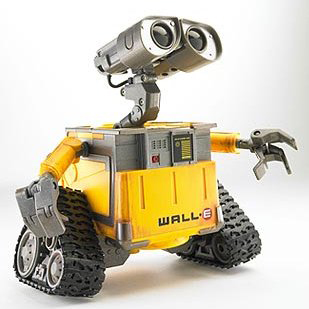
\includegraphics[width=0.33\textwidth]{images/robot.jpg}
	\caption{Base@Home Robot}%
	\label{fig:base_athome}
\end{wrapfigure}

Base@Home is a custom open-platform service robot developed by team UruBots for the RoboCup@Home Open Platform League (OPL). Physical specifications are as follows:

\begin{itemize}
	\item \textbf{Dimensions \& Weight:} Footprint $0.48\,\text{m} \times 0.48\,\text{m}$, chassis height $0.22\,\text{m}$, total height $1.35\,\text{m}$ (RuleBook \S 4.4: width $\le 70\,\text{cm}$, height $\le 200\,\text{cm}$). [TBD \#6: Measured total weight in kg].
	\item \textbf{Base Traction:} Differential-drive chassis ($0.48\,\text{m} \times 0.48\,\text{m}$, clearance $0.04\,\text{m}$). Two repurposed 6.5-inch brushless DC (BLDC) hub motors with Hall-effect sensors (15 pole pairs, 90 ticks/rev, $5.95\,\text{mm}$/tick), effective wheel radius $0.0853\,\text{m}$, track width $0.5620\,\text{m}$, rear passive caster wheel ($r = 0.04\,\text{m}$). STM32F103 motor controller with custom Field-Oriented Control (FOC) firmware~\cite{feru2024hoverboard} over UART at 50\,Hz. Maximum nominal velocity $0.38\,\text{m/s}$.
	\item \textbf{Torso (Pan-Elevation):} $1.30\,\text{m}$ central vertical aluminum profile ($0.06\,\text{m}$ width). NEMA 23 stepper motor (1600 steps/rev, 1/8 microstepping) driven by ESP32-S3 microcontroller with dual debounced hardware limit switches (working stroke $0.60\,\text{m}$, carriage height $0.40$--$1.00\,\text{m}$ above floor). Structural torso prism ($0.25\,\text{m} \times 0.35\,\text{m} \times 0.35\,\text{m}$) carrying a front-facing $0.26\,\text{m} \times 0.18\,\text{m}$ interactive facial display and speaker.
	\item \textbf{Manipulators (1):} Side-mounted AgileX Piper 6-DOF robotic arm ($1.5\,\text{kg}$ payload, $626\,\text{mm}$ reach, parallel two-finger gripper $0$--$95\,\text{mm}$) mounted on left vertical torso face ($+Y$ outward, $-Z$ downward). Shoulder origin at $z = 0.465$--$1.065\,\text{m}$ in base frame. Controlled via SocketCAN at 50\,Hz.
	\item \textbf{Head (Pan-Tilt):} 2-DOF pan-tilt unit driven by Robotis Dynamixel XL430-W250 servos over 1\,Mbaud U2D2 interface (IDs 1 and 2, Protocol 2.0, 20\,Hz).
	\item \textbf{RGB-D Sensors (2):}
		\begin{enumerate*}[label=(\roman*)]
			\item Intel RealSense D435 ($640\times 480$ @ 15\,Hz, firmware 5.17.0.10) mounted on the pan-tilt head;
			\item Orbbec DaBai DC1 ($640\times 480$ @ 15\,Hz) mounted eye-in-hand on the Piper wrist ($25\,\text{mm}$ along $+X$, $56\,\text{mm}$ above approach axis, $80\,\text{mm}$ behind fingertips).
		\end{enumerate*}
	\item \textbf{LiDAR Sensors (1):} Front Hokuyo UST-05LX 2D LiDAR ($270^\circ$ FOV, $0.06$--$5.0\,\text{m}$, 40\,Hz) at $x = 0.22\,\text{m}$, beam height $0.38\,\text{m}$.
	\item \textbf{Microphones (1):} Directional supercardioid shotgun microphone: R\O{}DE VideoMic GO II (USB, 48\,kHz capture downsampled to 16\,kHz) mounted on the head assembly.
	\item \textbf{Other Sensors:} Integrated Hall effect wheel sensors (90 ticks/rev); dual hardware limit switches on torso carriage; CAN feedback on Piper joints and gripper width.
	\item \textbf{Other Actuators:} ESP32-S3 stepper driver; parallel two-finger gripper ($0$--$95\,\text{mm}$).
	\item \textbf{Onboard Computing:}
		\begin{itemize}[nosep]
			\item Primary Host: CHUWI LarkBox S mini-PC (Intel Core i3-1220P 10C/12T, 15\,GiB RAM, 468\,GB NVMe SSD, Ubuntu 24.04.3 LTS, ROS 2 Jazzy). Runs navigation, planning, compiler, local LLM/VLM, and user interfaces.
			\item Secondary Host: NVIDIA Jetson Orin Nano 8\,GB Super Dev Kit (6-core Arm Cortex-A78AE, Ampere GPU, CUDA 13.2, TensorRT 10.16.2, 7.4\,GiB shared RAM, Ubuntu 24.04.4 LTS / JetPack 7.2.1). Runs arm controller, head controller, wrist vision, TensorRT YOLO inference, and streaming Whisper ASR.
		\end{itemize}
	\item \textbf{Internal Network:} Point-to-point 1\,Gbps wired Ethernet link ($0.2\,\text{ms}$ RTT, $\ge 660\,\text{Mbps}$) with unicast CycloneDDS (strictly no WiFi hotspot).
	\item \textbf{Power \& Safety:} [TBD \#7: Battery capacity, nominal voltage, BMS, fuse ratings, and emergency stop button per RuleBook \S 3.3.2].
\end{itemize}

\section*{Robot's Software Description}
\textit{Software packages developed specifically by team UruBots are marked with an asterisk ($^*$):}

\begin{itemize}
	\item \textbf{Audio filtering:} Silero VAD (voice activity detection), directional weak-voice gating ($0.34\,\text{ms}$/block).
	\item \textbf{Automated speech recognition:} \texttt{whisper\_node}$^*$ using \texttt{faster-whisper} (\texttt{base.en} int8 on CPU), request-indexed streaming pipeline, bilingual support.
	\item \textbf{Natural Language Processing:} \texttt{command\_parser.py}$^*$ (deterministic bilingual grammar DAG compiler), \texttt{gpsr\_parser}$^*$ / \texttt{gpsr\_plan.py}$^*$ (official GPSR grammar compiler), \texttt{llm\_intent.py}$^*$ (Qwen2.5 1.5B Q4 grammar-bounded fallback), \texttt{vlm.py}$^*$ / \texttt{vlm\_server.py}$^*$ (SmolVLM 500M Q8 for scene VQA).
	\item \textbf{Navigation, localization, and mapping:} Nav2~\cite{macenski2020marathon2} (AMCL, SmacPlanner2D, RegulatedPurePursuitController, RotationShimController), \texttt{hoverboard\_driver}$^*$, \texttt{front\_dock.py}$^*$ (LiDAR-based frontal docking), \texttt{map\_zone\_editor.py}$^*$ (semantic annotations).
	\item \textbf{Object recognition:} \texttt{bag\_finder.py}$^*$, YOLOv8s-worldv2~\cite{cheng2024yoloworld} open-vocabulary detector with background distractors, wrist DaBai DC1 monocular mid-height raycaster.
	\item \textbf{People recognition:} Face tracking with pan-tilt head; person Re-ID [TBD / future work].
	\item \textbf{People tracking:} YOLOv8n-pose with rolling torso-center tracking, \texttt{follow\_logic.py}$^*$ (distance-bounded person follower).
	\item \textbf{Pose/Gesture recognition:} 3D pointing-gesture localization (\texttt{bag\_vision.py}$^*$ raycasting arm-torso angle $\ge 25^\circ$), customer raised-hand detection (\texttt{raised\_hand.py}$^*$).
	\item \textbf{Manipulation:} \texttt{piper\_arm\_controller.py}$^*$ (50\,Hz SocketCAN with safety guards), \texttt{arm\_manipulation.py}$^*$, MoveIt 2 (TRAC-IK, OMPL multi-orientation planning), \texttt{door\_open.py}$^*$ (lever door opener), \texttt{quest\_teleop\_node.py}$^*$ (WebXR 6D pose Cartesian control).
	\item \textbf{Sound source localization:} None (directional shotgun mic with mechanical pan-tilt orientation).
	\item \textbf{Simulation Stack:} \texttt{base\_athome\_sim}$^*$ (\texttt{sim\_scene.py}$^*$ z-buffer RGB-D visual simulation, \texttt{sim\_arm.py}$^*$, \texttt{sim\_torso.py}$^*$, \texttt{sim\_mic.py}$^*$).
\end{itemize}

\section*{External Devices and Cloud Services}
\begin{itemize}
	\item \textbf{Wireless / Hotspots:} None (strictly zero-hotspot compliance per RuleBook \S 3.2.8~\cite{robocup_rulebook_2026}).
	\item \textbf{External Compute:} None. All planning, vision, ASR, foundation models, and control run 100\% onboard.
	\item \textbf{Development Teleoperation:} Meta Quest 2 headset via wired USB tunnel (\texttt{localhost:8765}).
	\item \textbf{Cloud Services:} None (no off-board or cloud APIs in the operational loop).
\end{itemize}


\nocite{*}

\end{document}
